\documentclass[a4paper,10pt,twocolumn]{extarticle}
\usepackage[T1]{fontenc}
%\usepackage[utf8]{inputenc}
\usepackage{lmodern}
\usepackage[francais]{babel}
\usepackage{textcomp}
\usepackage[top=2cm,bottom=2cm,left=2cm,right=2cm]{geometry}
\usepackage{amsmath}
\usepackage{amssymb}
\usepackage{mathrsfs}
\usepackage{float}
\usepackage{icomma}
\usepackage{gensymb}
\usepackage{graphicx}
\usepackage{subcaption}
\usepackage[font=sf, labelfont={sf,bf}, margin=1cm]{caption}
\usepackage[french,onelanguage,ruled,lined]{algorithm2e} % pour pseudo code
\usepackage{array}
\usepackage{titlesec, fontspec, titling}

% Specify different font for section headings
\newfontfamily\headingfont[]{GillSans}
\titleformat*{\section}{\LARGE\headingfont}
\titleformat*{\subsection}{\Large\headingfont}
\titleformat*{\subsubsection}{\large\headingfont}
\renewcommand{\maketitlehooka}{\headingfont}

\pretitle{\begin{flushleft}\fontsize{22}{18}}
\posttitle{\par\end{flushleft}\vskip 0.5em}
\preauthor{\begin{flushleft}\Large \lineskip 0.5em}
\postauthor{\par\end{flushleft}}
%\predate{\begin{flushleft}\large}
%\postdate{\par\end{flushleft}}
\setlength{\droptitle}{-1cm}
\title{\textsf{Implémantation d’un système de détection et de reconnaissance faciale}}
\author{Alexandre Bonhomme\\ {\normalsize Université Paul Sabatier, Toulouse}\\
Florent Maufras\\ {\normalsize EFREI, Paris}\\
Timothée Planté\\ {\normalsize EISTI, Pau}\\}% \small{BONA20128906}}
\date{}

\begin{document}
\maketitle
\section{Introduction}
La reconnaissance faciale est actuellement un domaine en plein essort. Elle rentre petit à petit dans nos vies au travers de nos téléphones mobiles ou de nos ordinateurs portables par exemple. Malgré l'amélioration du taux de détection elle reste l'objet de nombreuses études actuellement.

L'objectif de notre projet sera de mettre en oeuvre un système complet permettant la détection et la recnnaissance de visage issue de plusieurs bases de données. Pour ce faire nous implémenterons différents algorithmes de reconnaissances et nous utiliserons la bibliothèque OpenCV \cite{opencv} et son implémentation de l'algorithme de Viola \& Jones pour la détection de visage.

\section{Algorithmes mis en oeuvre}
Au cours de notre projet nous avons confronté différents algorithmes afin de tester leurs aptitudes sur plusieurs ensembles de donnée différents.

\subsection{K Plus Proches Voisins et Fenêtres de Parzen}
L'algorithme des <<K plus proches voisins>> (KPPV) utilise le voisinage du point de test afin de déterminer ça classe. C'est la classe majoritaire parmis ces $K$ points qui sera attribuée au point de test (\ref{fig:knn}).

Pour cet algorithme il n'y à pas d'apprentissage des paramètres sur l'ensemble d'entrainement, seulement une optimisation des l'hyperparamètres $K$ sur l'ensemble de validation.
\begin{figure}[H]
  \begin{center}
    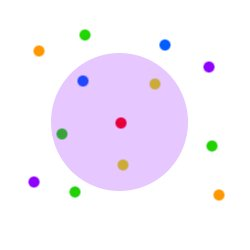
\includegraphics[width=100pt]{images_rapport/KNN.png}
    \caption{K Plus Proches Voisins}
    \label{fig:knn}
  \end{center}
\end{figure}
Dans la Figure~\ref{fig:knn} le point de test (en rouge) va recevoir comme prédiction la classe jaune car c'est elle la plus présente dans les $K = 4$ voisins les plus proches. Le disque ici n'est que représentatif pour mettre en évidence les voisins. Les points voisins pouvant être à une distance plus ou moins importantes de notre point test.

\subsubsection{Extension avec les fenêtres de Parzen}
L'application que l'on à fait ici de Parzen nous permet de pondéré les points du voisinage. Plus un point sera distant du point à l'étude plus sont poids sera faible. Cela est calculé à partir d'une gaussienne centrée sur le point à l'étude et d'une largeur fixé par $\sigma$, dans notre cas $\sigma$ sera fixé par l'utilisateur.

\subsection{Réseau de Neurones}
Le réseau de neurone utilisé dans ce projet est de type Perceptron Multicouche. Ce modèle est entrainé par descente de gradient de bacth sur un ensemble d'entrainement afin d'optimiser les paramètres du réseau en réduisant le risque empirique régularisé. On tâchera ensuite d'optimiser les hyperparamètres de contrôle de capacité sur un ensemble de validation séparé.
\begin{figure}[H]
  \begin{center}
    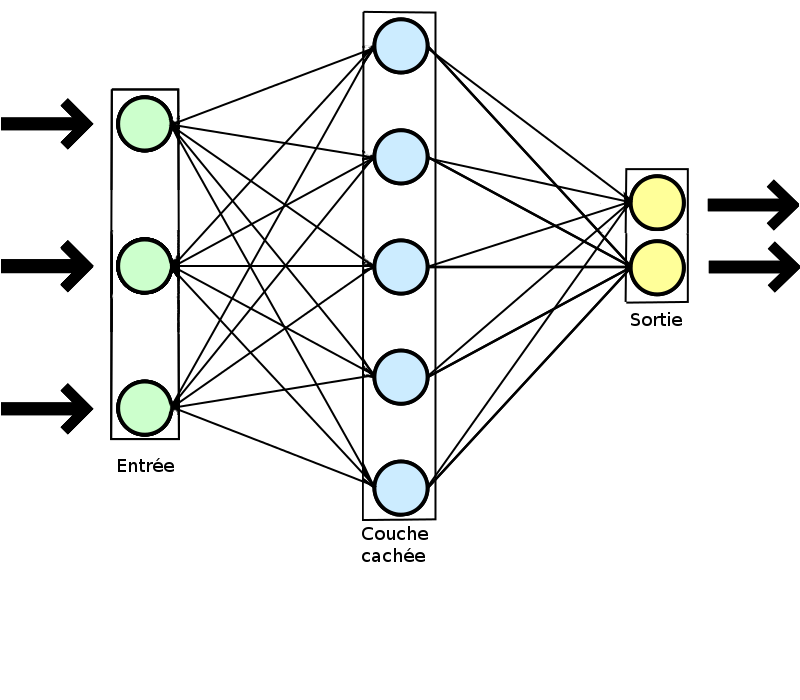
\includegraphics[width=220pt]{images_rapport/Neural_network.png}
    \caption{Réseau de neurones}
    \label{fig:nnet}
  \end{center}
\end{figure}
Dans notre cas nous utiliserons une architechture monocouche (cf. Figure~\ref{fig:nnet}) et une pénalité de type <<weight decay>> (\ref{eq:penalité}) pour la régularisation car elle défavorisera les poids les plus lourds lors de l'apprentissage des paramètres. 
\begin{align}\label{eq:penalité}
  \Omega(\theta) = \| \mathbf{W}^{(1)} \|^2 + \| \mathbf{W}^{(2)} \|^2
\end{align}
Cette pénalité sera pondérée par un hyperparamètre $\lambda$.

\subsection{Algorithme de Viola et Jones}
Afin d'effectué efficassement la détection de visage nous avons utilisé une implémentation de l'algorithme de Viola et Jones \cite{viola01} proposé par la célèbre bibliothèque de traitement d'image \textit{OpenCV} \cite{opencv}.

Cet algorithme est basé sur le principe de <<boosting>> qui conciste à assembler plusieurs classifieurs faibles afin d'obtenir un classifieur à forte capacité. Plutôt que de travailler directement sur les pixel de l'image, Viola P. et Jones M., introduise des caractéristique appelées <<pseudo-Haar>> fortement inspirées des ondelettes de Haar. De plus il utilise une variante d'un algorithme de boosting très célèbre qui est l'<<AdaBoost>>.
\begin{figure}[H]
        \centering
        \begin{subfigure}[b]{110pt}
                \centering
                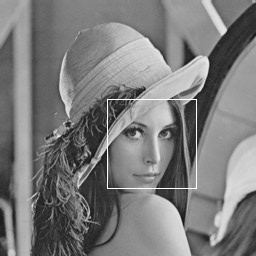
\includegraphics[width=110pt]{images_rapport/lena.png}
                \caption{Image initiale}
                \label{fig:lena}
        \end{subfigure}
        \begin{subfigure}[b]{110pt}
                \centering
                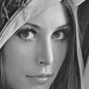
\includegraphics[width=60pt]{images_rapport/lena_face.png}
                \caption{Visage extrait}
                \label{fig:lena_face}
        \end{subfigure}
        \caption{Détection d'un visage par l'algorithme de Viola et Jones \cite{viola01} \label{fig:viola_detect}}
\end{figure}
Cette technique est particulièrement efficace et offre d'excelents résultats pour la détection de visages (cf. Figure~\ref{fig:viola_detect}) et par extention la détection de motifs (ou d'objets) au sein d'une image.

\section{Ensembles de données utilisés}
Afin d'entrainer nos algorithme et de mesurer leurs perfomance nous avons essentiellement utilisé deux jeux de données.

\subsection{Our Database of Faces (ORL \cite{orl})}
Le premier ensemble de donnée utilisé est issu des laboratoire de l'entreprise \textit{AT\&T}. C'est un ensemble de taille moyenne qui regroupe au total 40 sujets différent avec 10 images par sujets. Les photos on été prise sous différentes postures et durant plusieurs années et on une taille de $92 \times 112$ pixels.

Les images sont en niveaux de gris (NdG) et au format PGM.

\subsection{Labeled Faces in the Wild Home (LFW \cite{lfw})}
Pour le second jeu de données, il est mis a diposition par l'université du Massachusetts et il s'agit de photographies tirées d'Internet et sur lesquels l'algorithme de Viola et Jones \cite{viola01} a été appliqué afin d'obtenir une image de taille $250 \times 250$ pixels centré sur le visage.

Cet ensemble est relativement grand puis-ce qu'il contient 13233 images de 5749 sujets différents. Les images sont en couleur et au format JPG.

\subsection{Prétraitements des données}
\subsubsection{Cas particulier : l'ensemble LFW}
Contrairement à l'ensemble ORL, LFW nécéssite des prétraitement supplémentaires. En effet, nous avons utilisé l'ensemble LFW pour simuler une entrée réel dans noter système. Pour ce faire nous avons appliqué l'algorithme de Viola et Jones afin de détecter les visages au sein des images présentes dans l'ensemble.\\
Nous avons ainsi pu extraire (après divers traitements de redimentionnement) une image de taille $92 \times 115$ pixels en plusieurs NdG.

\subsubsection{Cas général}
Appartir des images en différents NdG nous construisons une représentation vectoriel de celle-ci (cf. Figure~\ref{fig:vectorisation}).
\begin{figure}[H]
  \begin{center}
    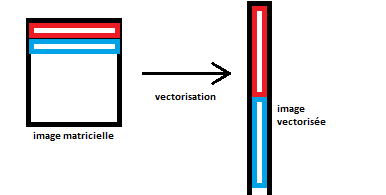
\includegraphics[width=220pt]{images_rapport/vectorisation.png}
    \caption{Vectorisation d'une image}
    \label{fig:vectorisation}
  \end{center}
\end{figure}
Cependant cette représentation est très lourde car elle contient de nombreuses caractéristiques. Afin de reduire la dimentionailé de nos données d'entraienement nous avons appliqué l'agorithme du \textit{PCA} (<<Principal Components Analysis>>), plus connu sous le nom de <<Eigenfaces>> \cite{turk91} lorsqu'il est appliqué à la reconnaissance facial.

\subsubsection{Réduction de la dimentionnalité : PCA}
Nous avons implémenté le PCA dans ca forme classique.\\
On normalise l'ensemble de donnée en sustraillant le <<visage>> moyen :
\begin{align}
  X_N = X - \bar{x}
\end{align}
A la suite de quoi nous utilisons une <<astuce mathématique>> qui consiste à calculer la Décomposition en Valeurs Singulières (ou SVD pour <<Singular Value Decomposition>>) afin de déterminer les vecteurs propres de la matrice de covariance. On obtient alors :
\begin{align}
  X_N = USU^T
\end{align}
Ou les colonnes de $U$ contienent les vecteurs propres et $S^2$ les valeurs propres associées. On ne conserve alors qu'un nombre $M$ de vecteurs propres (ie. $M$ colonnes de la matrice $U$). Après réduction du nombre de colonne on obtient une matrice $U^{\prime}$ (aussi appelée, dans notre cas, <<Eigenspace>>) dans laquelle on projetent l'ensemble de donnée $X$ afin de déterminer la matrice de poids $W$ associée :
\begin{align}
  W = \langle (U^{\prime})^T , X \rangle
\end{align}
Ainsi, pour chaque nouvel exemple $x$ on calculera son vecteur de poids $w$ par projection dans dans le Eigenspace $U^{\prime}$.

\section{Vérifications des algorithmes}
Afin de vérifier le bon fonctionnement des algorithmes implémentés nous avons mis en oeuvre quelques procédures de vérification.

\subsection{Perceptron Multicouche}
Pour le réseau de neurones nous avons vérifié nos résultat sur l'ensemble de donnée deux dimenssions <<MOONS>> et nous avons obtenue les résultats de la Figure~\ref{fig:verif_nnet}.
\begin{figure}[H]
        \centering
        \caption{Vérification du réseau de neurones}\label{fig:verif_nnet}
        \begin{subfigure}[b]{220pt}
                \centering
                \caption{Risque empirique}
                \includegraphics[width=220pt]{images_rapport/nnet_risque.png}
        \end{subfigure}
        \begin{subfigure}[b]{220pt}
                \centering
                \caption{Erreur de classification}
                \includegraphics[width=220pt]{images_rapport/nnet_erreur_classif.png}
        \end{subfigure}
        \begin{subfigure}[b]{220pt}
                \centering
                \caption{Frontières de décision}
                \includegraphics[width=220pt]{images_rapport/nnet_fontieres.png}
        \end{subfigure}
\end{figure}

\subsection{Détection de visages}
Pour vérifier le bon fonctionnement de la détection de visage nous avons effectué des essaies préalable du des images de test tel que celle de la Figure~\ref{fig:viola_detect}.

\section{Résultats}
Afin d'évaluer la performance des deux algorithmes sur les deux ensembles de données nous les avons chacun divisés en trois lots de la manière suivante :
\begin{description}
  \item[60\%] Ensemble d'entrainement
  \item[20\%] Ensemble de validation
  \item[20\%] Ensemble de test
\end{description}
Les lots son généré de manière aléatoire à chaque lancement de l'application.

Pour chaque ensemble de test nous avons évalué l'algorithme du KNN et le Perceptron Multicouche avec différentes valeurs d'hyperparamètres.

\subsection{Ensemble ORL}
\begin{figure}[H]
  \begin{center}
    \includegraphics[width=220pt]{images_rapport/hist_orl.png}
    \caption{Meilleurs résultats pour l'ensemble ORL}
    \label{fig:results_orl}
  \end{center}
\end{figure}
Comme le montre la Figure~\ref{fig:results_orl} sur le jeu de donnée ORL l'algorithme du KNN est très performant avec pret de 90\% de précision pour $K = 1$. En revanche on observe que l'augmentation de nombre de voisins n'est pas très efficase, voir très inefficase pour un faible nombre d'exemples.

Le Réseau de Neurone quand à lui donne des résultats mitigés et parfois aléatoirement très mauvais. Les hyperparamètres sont beaucoup plus difficiles à optimiser car plus nombreux ce qui entraine parfois des résultats abérants. Nous n'avons pas réussit à optenir de bon résultats constants avec cet algorithme sur ce jeu d'entrainement.

En conclusion pour cet ensemble <<simple>> la technique des K plus proches voisins est de loin la meilleur et la plus stable avec un $K = 1$.

\subsection{Ensemble LFW}
L'ensemble LFW s'est avéré beaucoup plus difficile à appréander. En effet les images sont de moins bonnes qualités, les visages sont souvent de profil et peuvent comporter divers expressions.
\begin{figure}[H]
  \begin{center}
    \includegraphics[width=220pt]{images_rapport/ErrorKnnEx75LFW.png}
    \caption{Observation des résultats du KNN}
    \label{fig:knn_lfw}
  \end{center}
\end{figure}
Sur cet ensemble on vois clairement (cf. Figure~\ref{knn_lfw})que l'algorithme des K plus proches voisins est totalement inéfficasse. Celui-ci ne s'adapte pas du tout à cet ensemble compliqué à cause de ca faible capacité.

\begin{figure}[H]
  \begin{center}
    \includegraphics[width=220pt]{images_rapport/hist_lfw.png}
    \caption{Meilleurs résultats pour l'ensemble LFW}
    \label{fig:results_lfw}
  \end{center}
\end{figure}
Le réseaux de neurones donne des résultats plus prométeurs. Il nécessite en revanche un grand nombre d'image pour être efficase et atteindre un niveaude reconnaissance acceptable.

\section{Particularités du projet}
Une des caractéristiques de notre projet est qu'il a été réalisé par une équipe de trois personnes ayant suivient des formations différentes. De plus nous avons du mettre en place un gestionnaire de version (Git) afin de pouvoir travailler efficacement malgré nos diponibilités très disparates.

L'usage du langage Python à aussi ajouté son lot de complications car nous avons tous les trois découvert ce langage au début du semestre.

La dernière difficulté, et non des moindres, concerne le sujet en lui même. En effet, la reconnaissance faciale est encore un sujet d'étude actuellement et aucun système n'est encore réellement fiable dans ce domaine.

\section{Conclusion}


\begin{thebibliography}{9}
\bibitem{turk91}
  \bsc{Turk M. and Pentland A.}, 
  \emph{Eigenfaces for recognition}.
  J. Cognitive Neuroscience,
  1991. 
\bibitem{orl}
  \bsc{Samaria F. and
      Harter A.}, 
  \emph{Parameterisation of a stochastic model for human face identification}.
  2nd IEEE Workshop on Applications of Computer Vision,
  1994.
\bibitem{opencv}
  \bsc{Bradski G.}, 
  \emph{The OpenCV Library}.
  Dr. Dobb's Journal of Software Tools,
  2000.
\bibitem{viola01}
  \bsc{Viola P. and 
      Jones M.}, 
  \emph{Rapid object detection using a boosted cascade of simple features}.
  Computer Vision and Pattern Recognition,
  2001.
\bibitem{lfw}
  \bsc{Huang G. B.,
       Ramesh M.,
       Berg T. and 
       Learned-Miller E.}, 
  \emph{Labeled Faces in the Wild: A Database for Studying Face Recognition in Unconstrained Environments}.
  University of Massachusetts, Amherst,
  2007.

\end{thebibliography}
\end{document}
